\documentclass[../notmain.tex]{subfiles}
% \documentclass[class=exam,crop=false]{standalone}
% \usepackage{preambles}
% \usepackage[subpreambles=true]{standalone}

\loadallproblems{trigoprob.tex}

\begin{document}
\setup{Application of Trigonometry}{}
\fullwidth{\Large \textbf{Introduction}}
\begin{figure}[h]
    \centering
    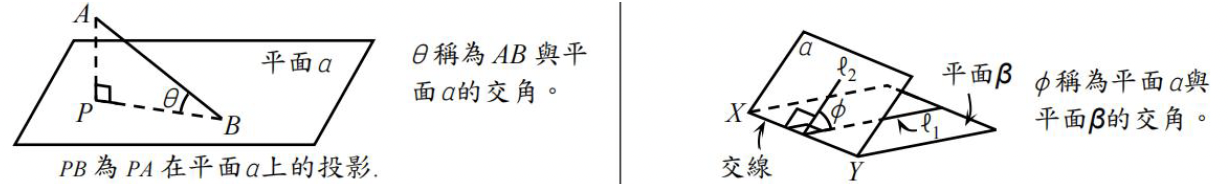
\includegraphics[width=1\linewidth]{assets/ddw13.png}
\end{figure}
\hrule
\bigskip
\fullwidth{\Large \textbf{Practice}}
    \begin{questions}
        \question 
        \adjustbox{valign=t,center}{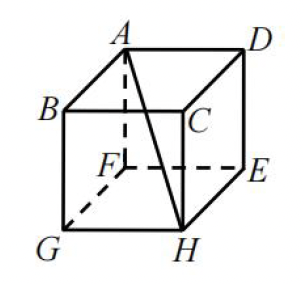
\includegraphics[width=0.25\linewidth]{assets/jdj2e.png}}
        In the figure, $ABCDEFGH$ is a cube.
        \begin{parts}
            \part Write down the projection of line $AH$ on different surfaces:
            \begin{subparts}
                \subpart $EFGH$   
                \subpart $ADEF$
            \end{subparts}
            \part Write down the angle between line $AH$ and surfaces:
            \begin{subparts}
                \subpart $ABGF$
                \subpart $ABCD$
            \end{subparts}
        \end{parts}
        \dlines{1}
        \clearpage
        \question
            \adjustbox{valign=t,center}{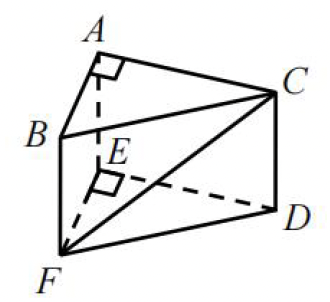
\includegraphics[width=0.25\linewidth]{assets/adijeod.png}}
            In the figure, $ABCDEF$ is a triangular pyramid and its base $ABC$ is a right angled triangle.
            \begin{parts}
                \part Write down the angle between CF and 
                \begin{subparts}
                    \subpart $ACDE$
                    \subpart $ABFE$
                    \subpart $ABC$
                \end{subparts}
                \part
                Write down angle between surface $BFDC$ and 
                \begin{subparts}
                    \subpart $ACDE$
                    \subpart $ABFE$
                \end{subparts}
            \end{parts}
        \dlines{1}
        \clearpage
        \question
        圖中是一個正立方體。$I$為$GD$上的一點。$DI:IG=1:2$ 和 $GJ:JB=1:2$。求 $IJ$和平面 $CGFB$ 之間的交角。\\The image depicts a regular cube. $I$ is a point on $GD$. Given that $DI:IG=1:2$ and $GJ:JB=1:2$, calculate the angle between $IJ$ and the plane $CGFB$.\par
        \begin{center}
            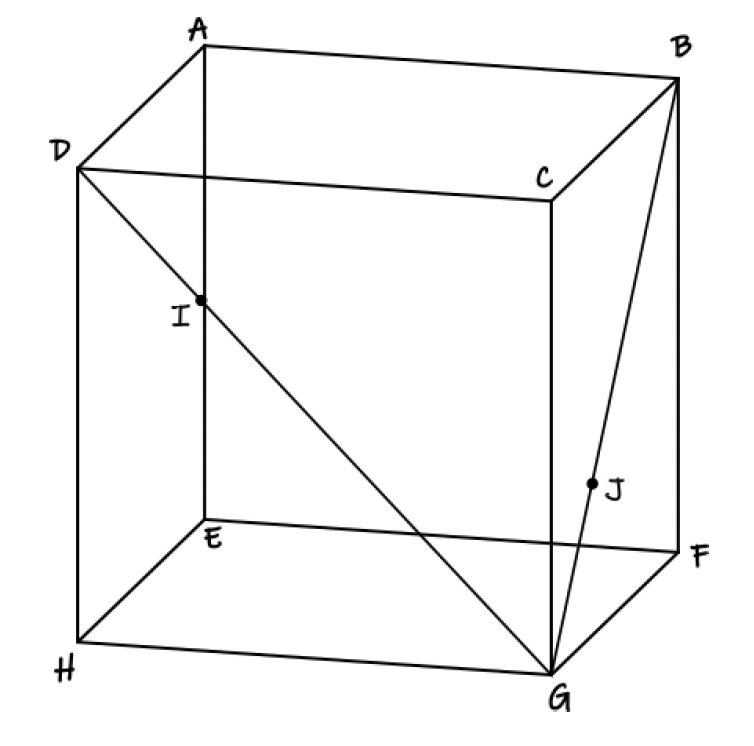
\includegraphics[width=0.4\linewidth]{assets/dwq2r.png}
        \end{center}
        \dlines{1}
        \clearpage
        \dlines{1}
            
    \end{questions}
\clearpage
\begin{questions}
    % \ansdisplay
\question 
    \useproblem{qone}
    \dlines{1}
    \clearpage
    \dlines{1}

\clearpage
\question
    \useproblem{qtwo}
    \dlines{1}
    \clearpage
    \dlines{1}

\clearpage
\question
    \useproblem{qthree}
    \dlines{1}
    \clearpage
    \dlines{1}

\clearpage
\question
    \useproblem{qfour}
    \dlines{1}
    \clearpage
    \dlines{1}

\clearpage
\question
    \useproblem{qfive}
    \dlines{1}
    \clearpage
    \dlines{1}



    
\end{questions}




















\end{document}